%!TEX root = ../Dimensionieren I.tex

\section{Nietverbindungen} % (fold)
	\subsection{Entwurfsrichtlinien} % (fold)
		Schwächungsverhältnis:
		\begin{equation*}
			V = \frac{\text{Nutzquerschnitt}}{\text{Vollquerschnitt}}=  \frac{b-z\cdot d}{b}, \hfill V \in [0.7 , 0.85]
		\end{equation*}
		mit $z$ als Anzahl Nieten.
		
		Nietdurchmesser $d'$ vor dem Schlagen:
		\begin{equation*}
			\text{Stahlbau} \hfill 1.3\cdot s \leq d' \leq 3 \cdot s
		\end{equation*}
		\begin{equation*}
			\text{Leichtmetallbau} \hfill 1.5 \cdot s \leq d' \leq 2.5 \cdot s
		\end{equation*}
		\begin{center}
			\begin{tabular}{llr}
				\toprule
				\textbf{Variable} & \textbf{Stahl- und Kranbau} & \textbf{Leichtmetallbau} \\
				\midrule
				$a$ & $15\cdot s \text{ bzw. } 6\cdot d \geq a \geq d$ & $6\cdot d \geq a \geq 2.5 \cdot d$\\
				$e$ & $8\cdot s \text{ bzw. } 4\cdot d \geq e \geq 2\cdot d$ & $e \geq 2 \cdot d$ \\
				$e'$ & $e' \geq 0.5 \cdot a$ & $e' \geq 2 \cdot d$\\
				\bottomrule
			\end{tabular}
		\end{center}
		
		\begin{center}
			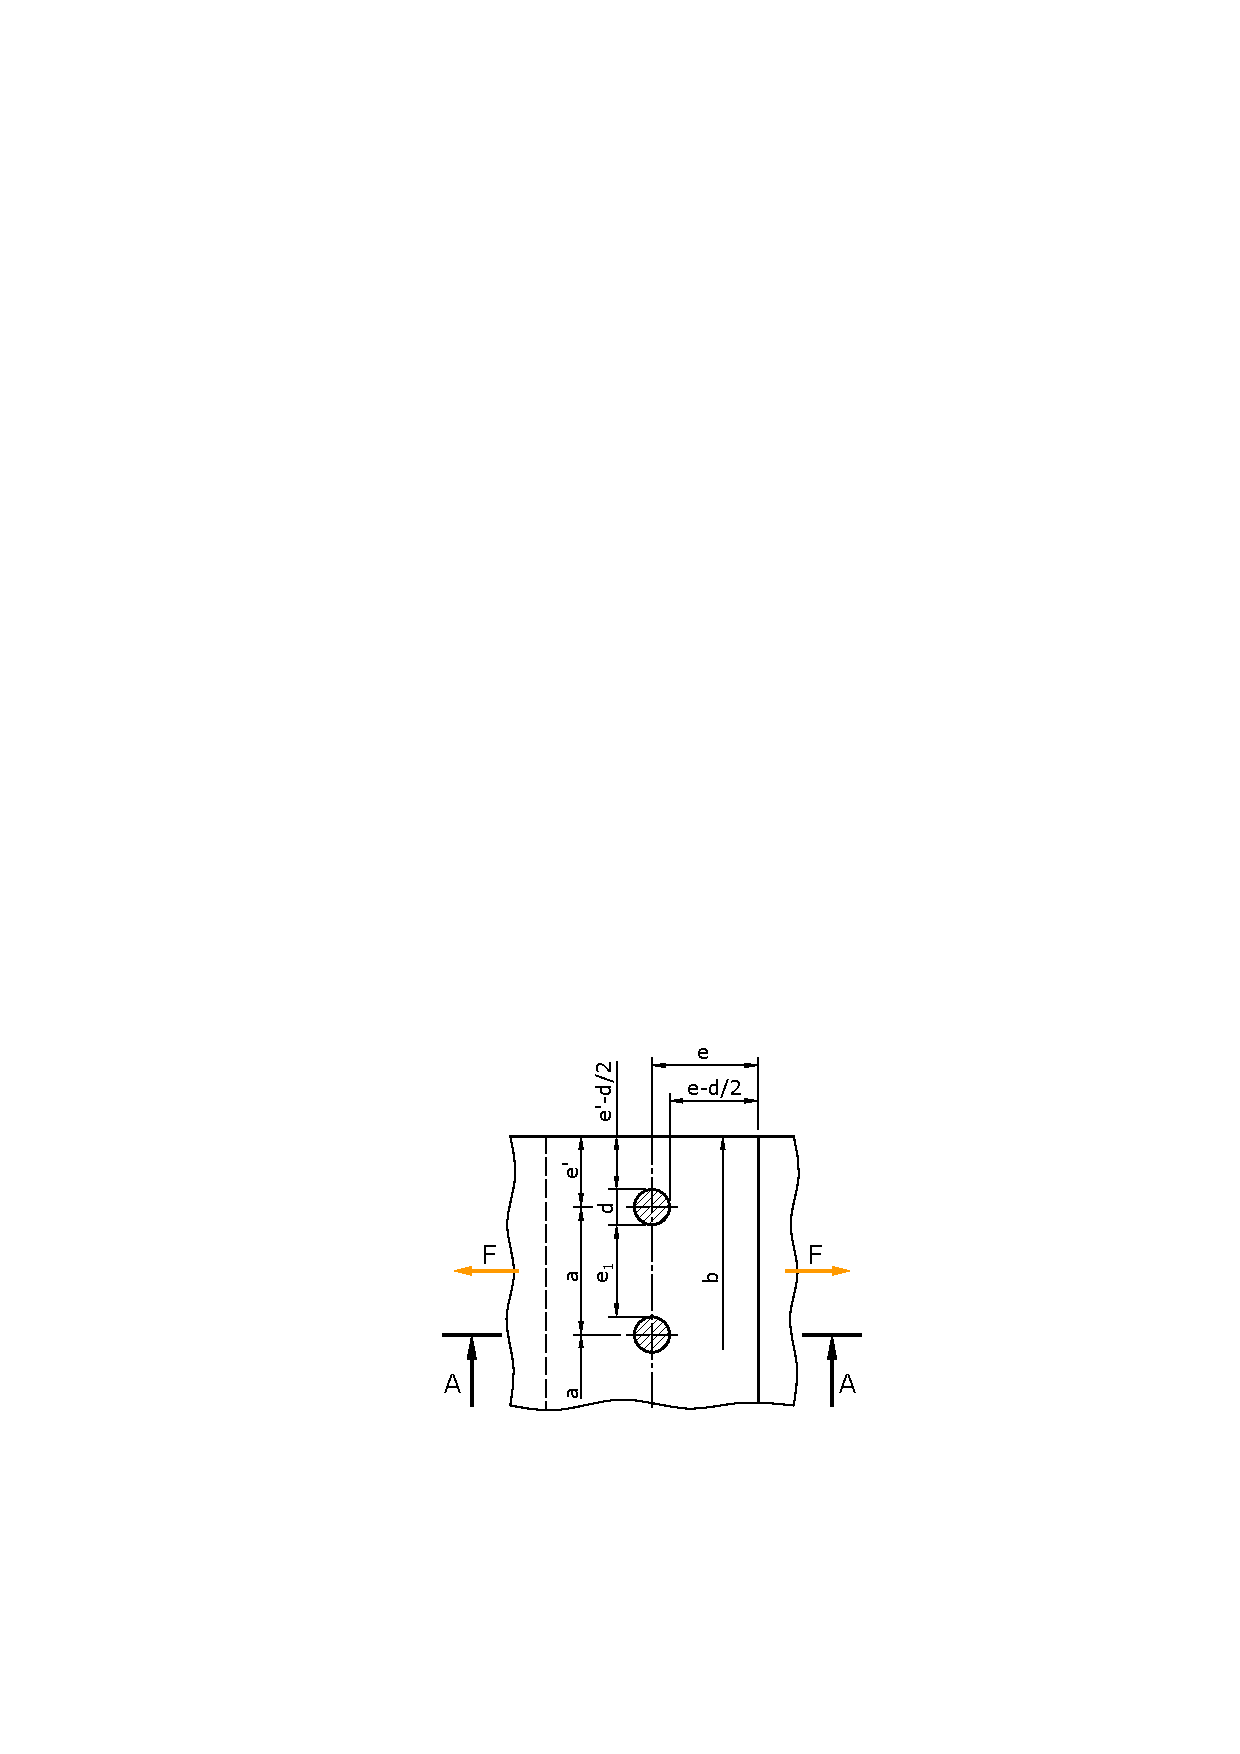
\includegraphics[width=.75\columnwidth]{graphics/niete_2}
		\end{center}
		
		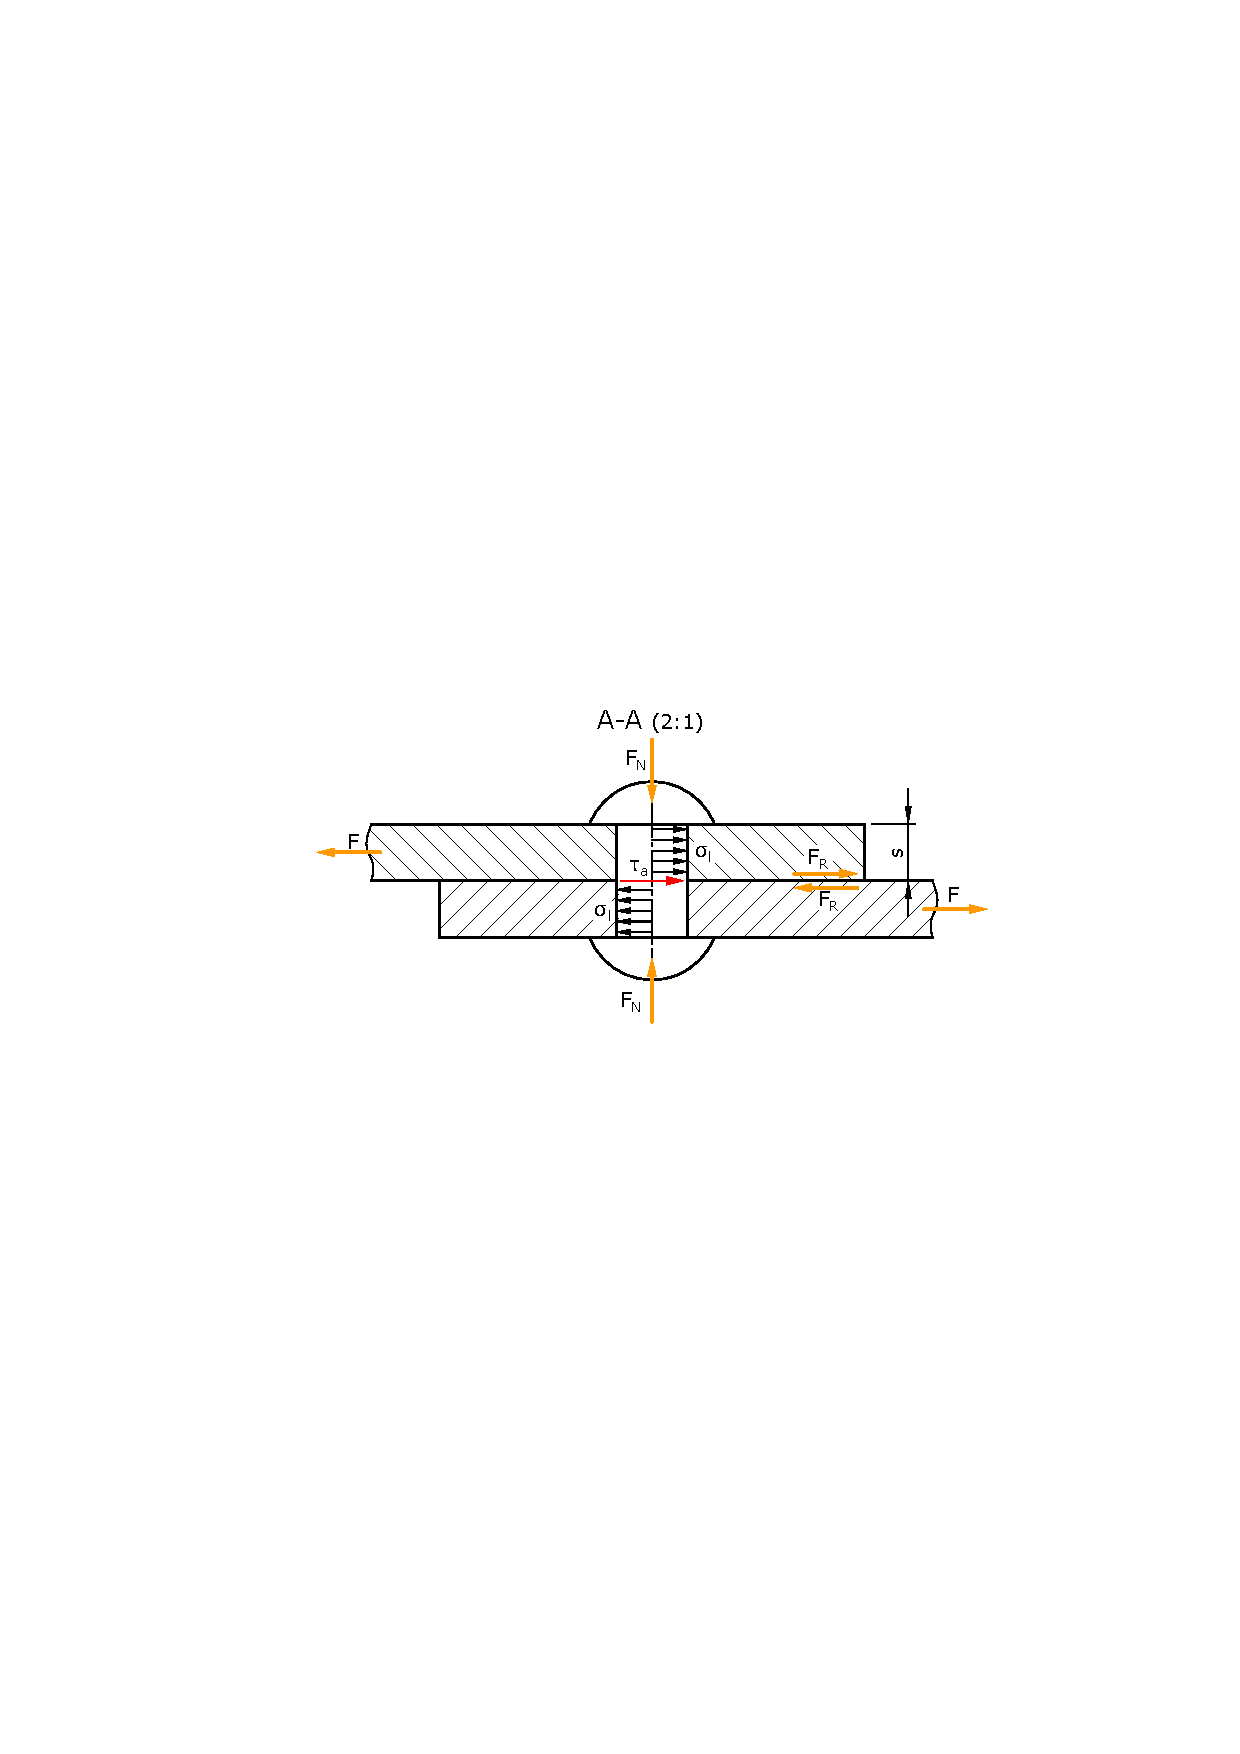
\includegraphics[width=\columnwidth]{graphics/niete_1}
	% subsection: Entwurfsrichtlinien (end)
	\subsection{Kraftschlüssige Nietverbindungen} % (fold)
		Bedingung:
		\begin{equation*}
			z\cdot F_{\text{R}} = z \cdot F_{\text{N}} \cdot \mu_0 \geq F
		\end{equation*}
		\begin{equation*}
			F_{\text{N}} = \sigma_{\text{z}}\cdot \underbrace{\frac{d^2\pi}{4}}_{A_{\text{N}}}, \quad F_{\text{R}}= \mu_0 \cdot  \sigma_{\text{z}} \cdot \frac{d^2\pi}{4} = k_n \cdot \frac{d^2\pi}{4}
		\end{equation*}
		\begin{equation*}
			k_n \leq \conditional{\SI{70}{\mega\pascal} & \text{USt 36-1 (S 253)}\\
				\SI{80}{\mega\pascal} & \text{RSt 44-2 (S 275)}}
		\end{equation*}
		\begin{equation*}
			z = \frac{F}{A_{\text{N}}\cdot k_n \cdot n}, \quad n = \text{Schnittigkeit}
		\end{equation*}
		
		\begin{equation*}
			\sigma_{\text{z}} = \frac{\alpha \cdot \Delta T \cdot E}{2} \leq \sigma_{\text{F}}, \hfill \Delta T = T_{\text{Schlagen}}-T_{\text{Umgebung}}
		\end{equation*}
	% subsection: Kraftschlüssige Nietverbindungen (end)
	\subsection{Formschlüssige Nietverbindungen} % (fold)
		\begin{enumerate}
		\item Beanspruchung des Niets
			\begin{enumerate}
				\item Scherspannung:
					\begin{equation*}
						\tau_a = \frac{F}{A_{\text{N}}\cdot z} \leq \tau_{a\text{,zul}}
					\end{equation*}
				\item Flächenpressung:
					\begin{equation*}
						\sigma_l = \frac{F}{d \cdot s \cdot z} \leq \sigma_{l\text{,zul}}
					\end{equation*}
				\item Erforderliche Anzahl Nieten:
					\begin{equation*}
						z = \frac{F}{d \cdot s \cdot \sigma_{l\text{,zul}}} = \frac{4F}{\pi \cdot d^2 \cdot \tau_{a\text{,zul}}}
					\end{equation*}
			\end{enumerate}
		\item Beanspruchung der Bauteile:
			\begin{enumerate}
				\item Lochleibung:
					\begin{equation*}
						\sigma_l = \frac{F}{d \cdot s \cdot z} \leq \sigma_{l\text{,zul}}
					\end{equation*}
				\item Normalspannung zwischen den Nieten:
					\begin{equation*}
						\sigma_z = \frac{F}{(b-z\cdot d)\cdot s} \leq \sigma_{l\text{,zul}}
					\end{equation*}
				\item Scherspannung zum Rand:
					\begin{equation*}
						\tau = \frac{F}{2\cdot z \cdot \left( e-\frac{d}{2}\right)\cdot s} \leq \tau_{\text{,zul}}
					\end{equation*}
				\item Biegebeanspruchung bei Überlappnietung:
					\begin{equation*}
						\sigma_{\text{B}} = \frac{M_b}{W_b} = \frac{3\cdot F}{b \cdot s}
					\end{equation*}
			\end{enumerate}
		\end{enumerate}
		Für zulässige Festigkeitswerte siehe Anhang \ref{flaechenbelastungen}.
	% subsection: Formschlüssige Nietverbindungen (end)
	\subsection{Momentenbelastete Nietverbindungen} % (fold)
		\begin{equation*}
			F_{\text{Niet}_{\text{max}}} = \max (F_{Qi}+F_{Mi}) = \max \left( \frac{F}{z} + \frac{M \cdot r}{\sum r_i^2}\right)
		\end{equation*}

		\paragraph{Nieten auf Teilkreis:} % (fold)
			~
			\begin{center}
				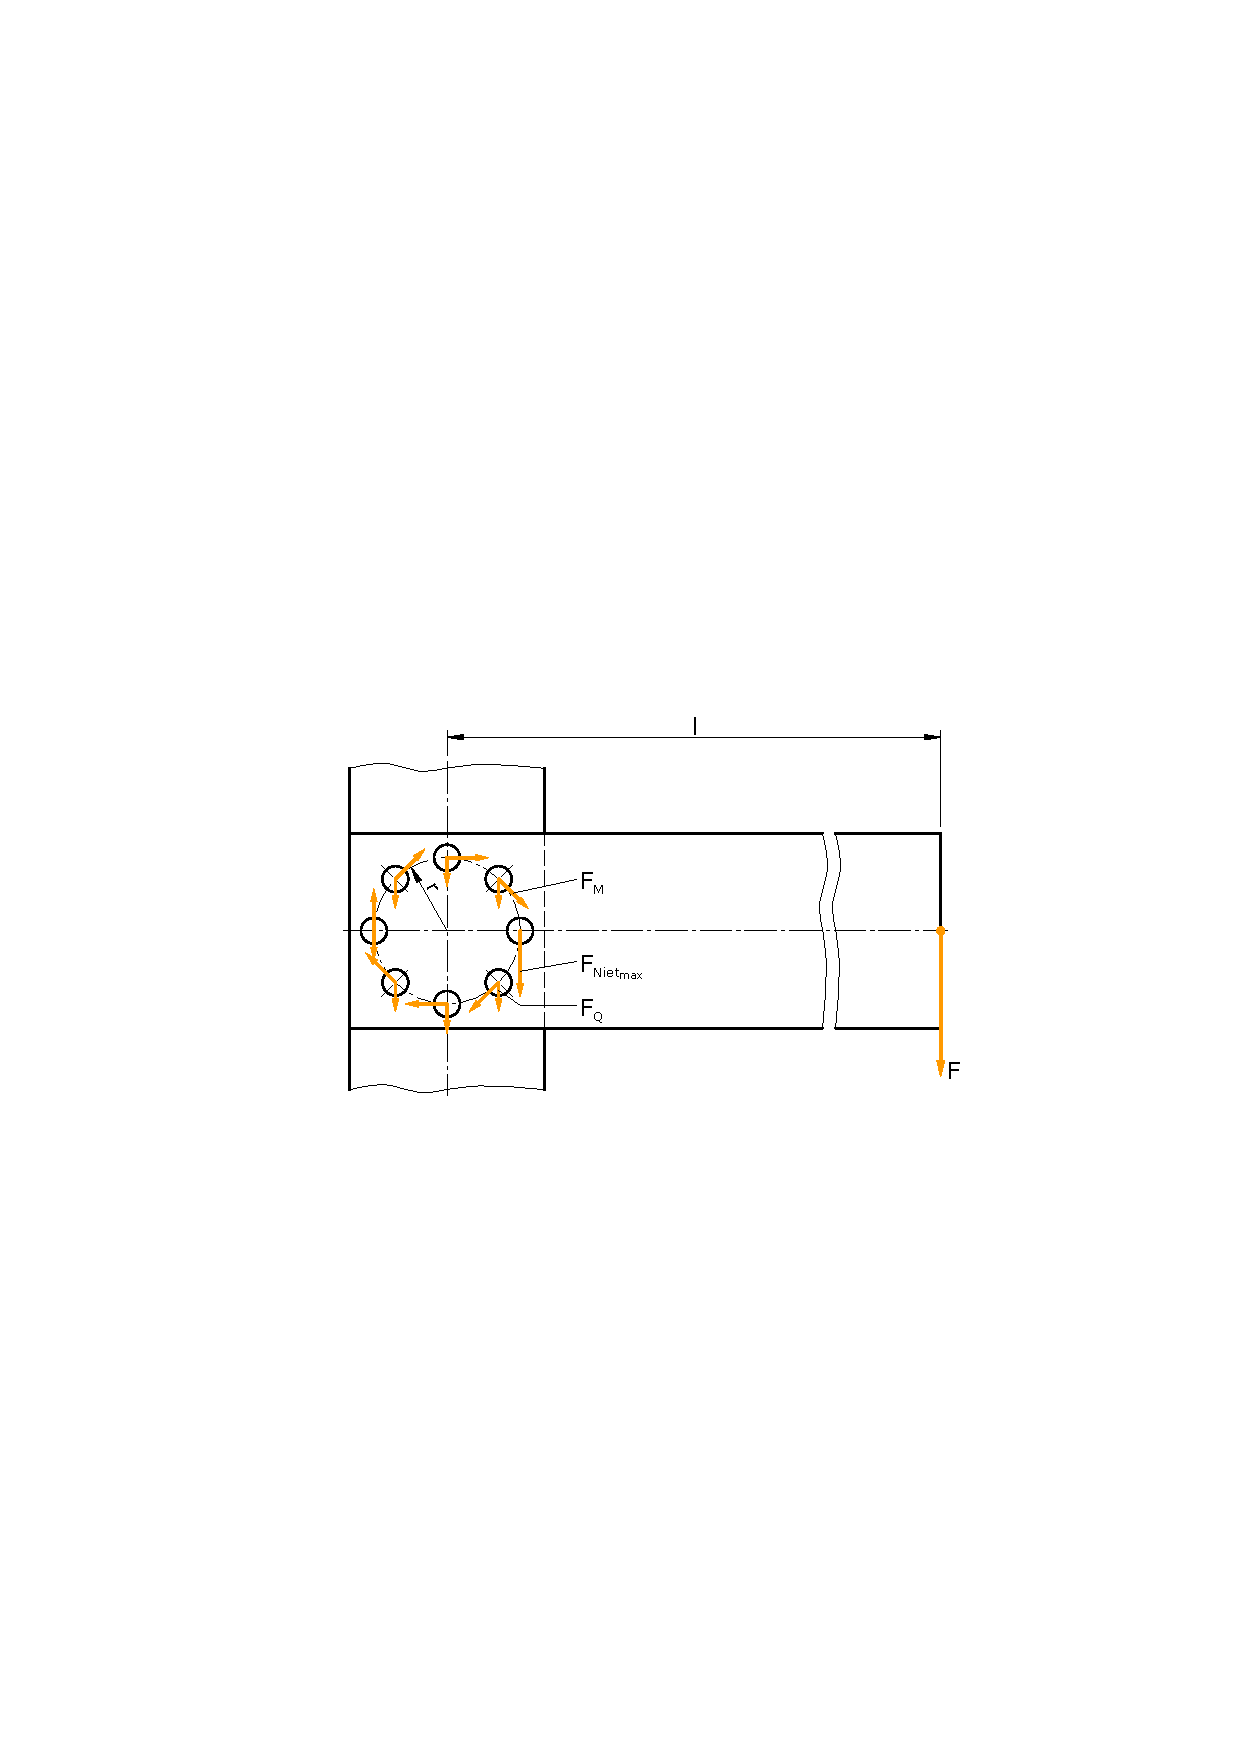
\includegraphics[width=\columnwidth]{graphics/nietenteilkreis}
			\end{center}
			\begin{equation*}
				F_{\text{Niet}_{\text{max}}} = \frac{F}{z} \cdot \left( 1 + \frac{l}{r}\right)
			\end{equation*}
		% paragraph: Nieten auf Teilkreis: (end)


		\paragraph{Nieten nicht auf Teilkreis:} % (fold)
			~
			\begin{center}
				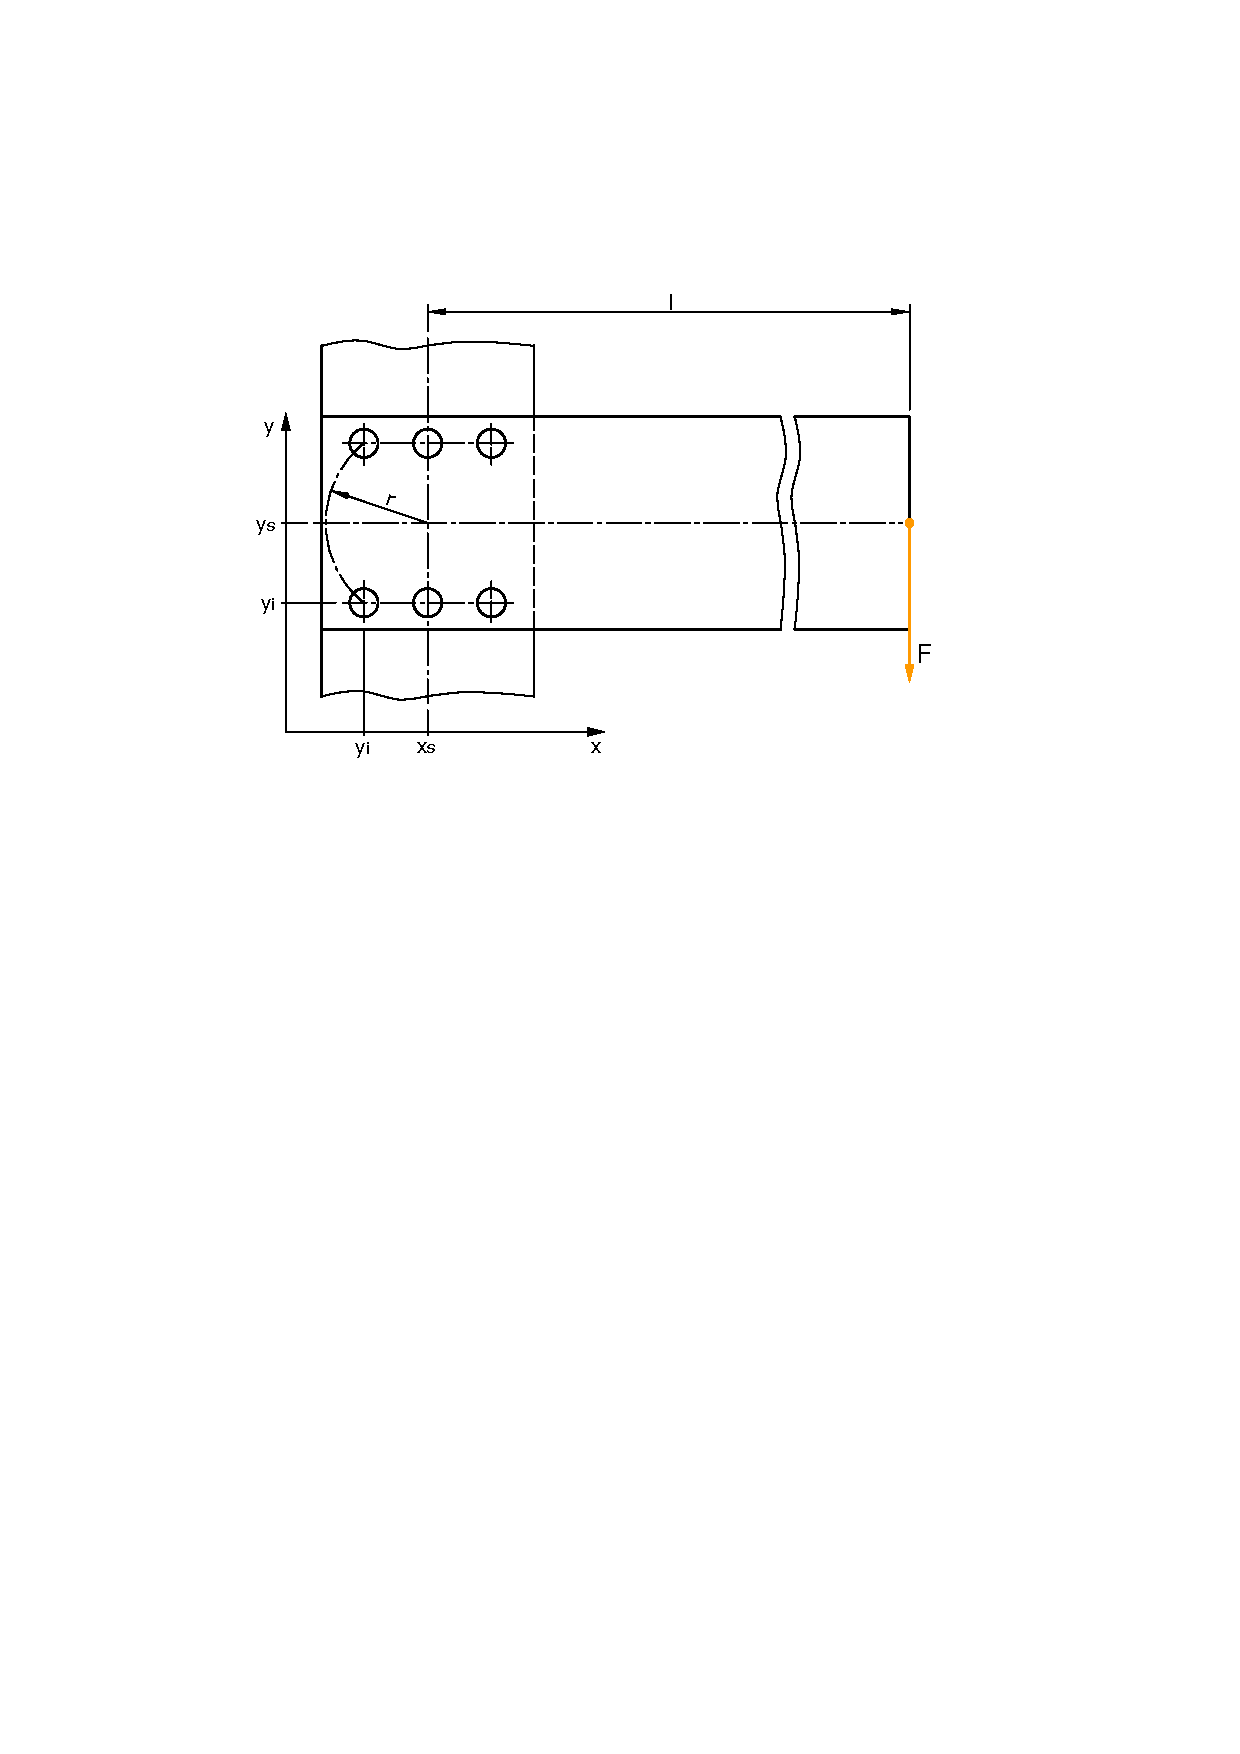
\includegraphics[width=\columnwidth]{graphics/nietennichtteilkreis}
			\end{center}
			\begin{enumerate}
				\item Schwerpunkt des Nietbildes bestimmen:
					\begin{equation*}
						x_S = \frac{1}{z} \sum_{i=1}^z x_i\ , \qquad y_S = \frac{1}{z} \sum_{i=1}^z y_i
					\end{equation*}
				\item Schwerpunktabstand $r_i$ aller Nieten bestimmen
				\item Nietbelastung aus Moment und Querkraft berechnen:
					\begin{equation*}
						F_{Mi} = \frac{F\cdot l \cdot r_i}{\sum_{j=1}^z r_j^2} \quad F_{Qi}=\frac{F}{z}
					\end{equation*}
				\item Grösste resultierende Nietkraft:
					\begin{equation*}
						F_{\text{Niet}_{\text{max}}} = \max (\vec F_{Qi}+\vec F_{Mi})
					\end{equation*}
			\end{enumerate}
		% paragraph: Nieten nicht auf Teilkreis: (end)
	% subsection: Momentenbelastete Nietverbindungen (end)
	\subsection{Gestaltungsrichtlinien} % (fold)
		\begin{tightitemize}
			\item Zugbeanspruchung des Niets verhindern.
			\item Mindestens 2 Niete pro Bauteil.
			\item Bei Überlappungsnietung Biegemoment beachten.
			\item Doppellaschennietung bevorzugen (Kein Biegemoment, besseres Schwächungsverhältnis).
		\end{tightitemize}
	% subsection: Gestaltungsrichtlinien (end)
% section: Nietverbindungen (end)
\section{Stift- und Bolzenverbindungen} % (fold)
	\subsection{Querkraftbelastete Steckstifte} % (fold)
		\begin{center}
			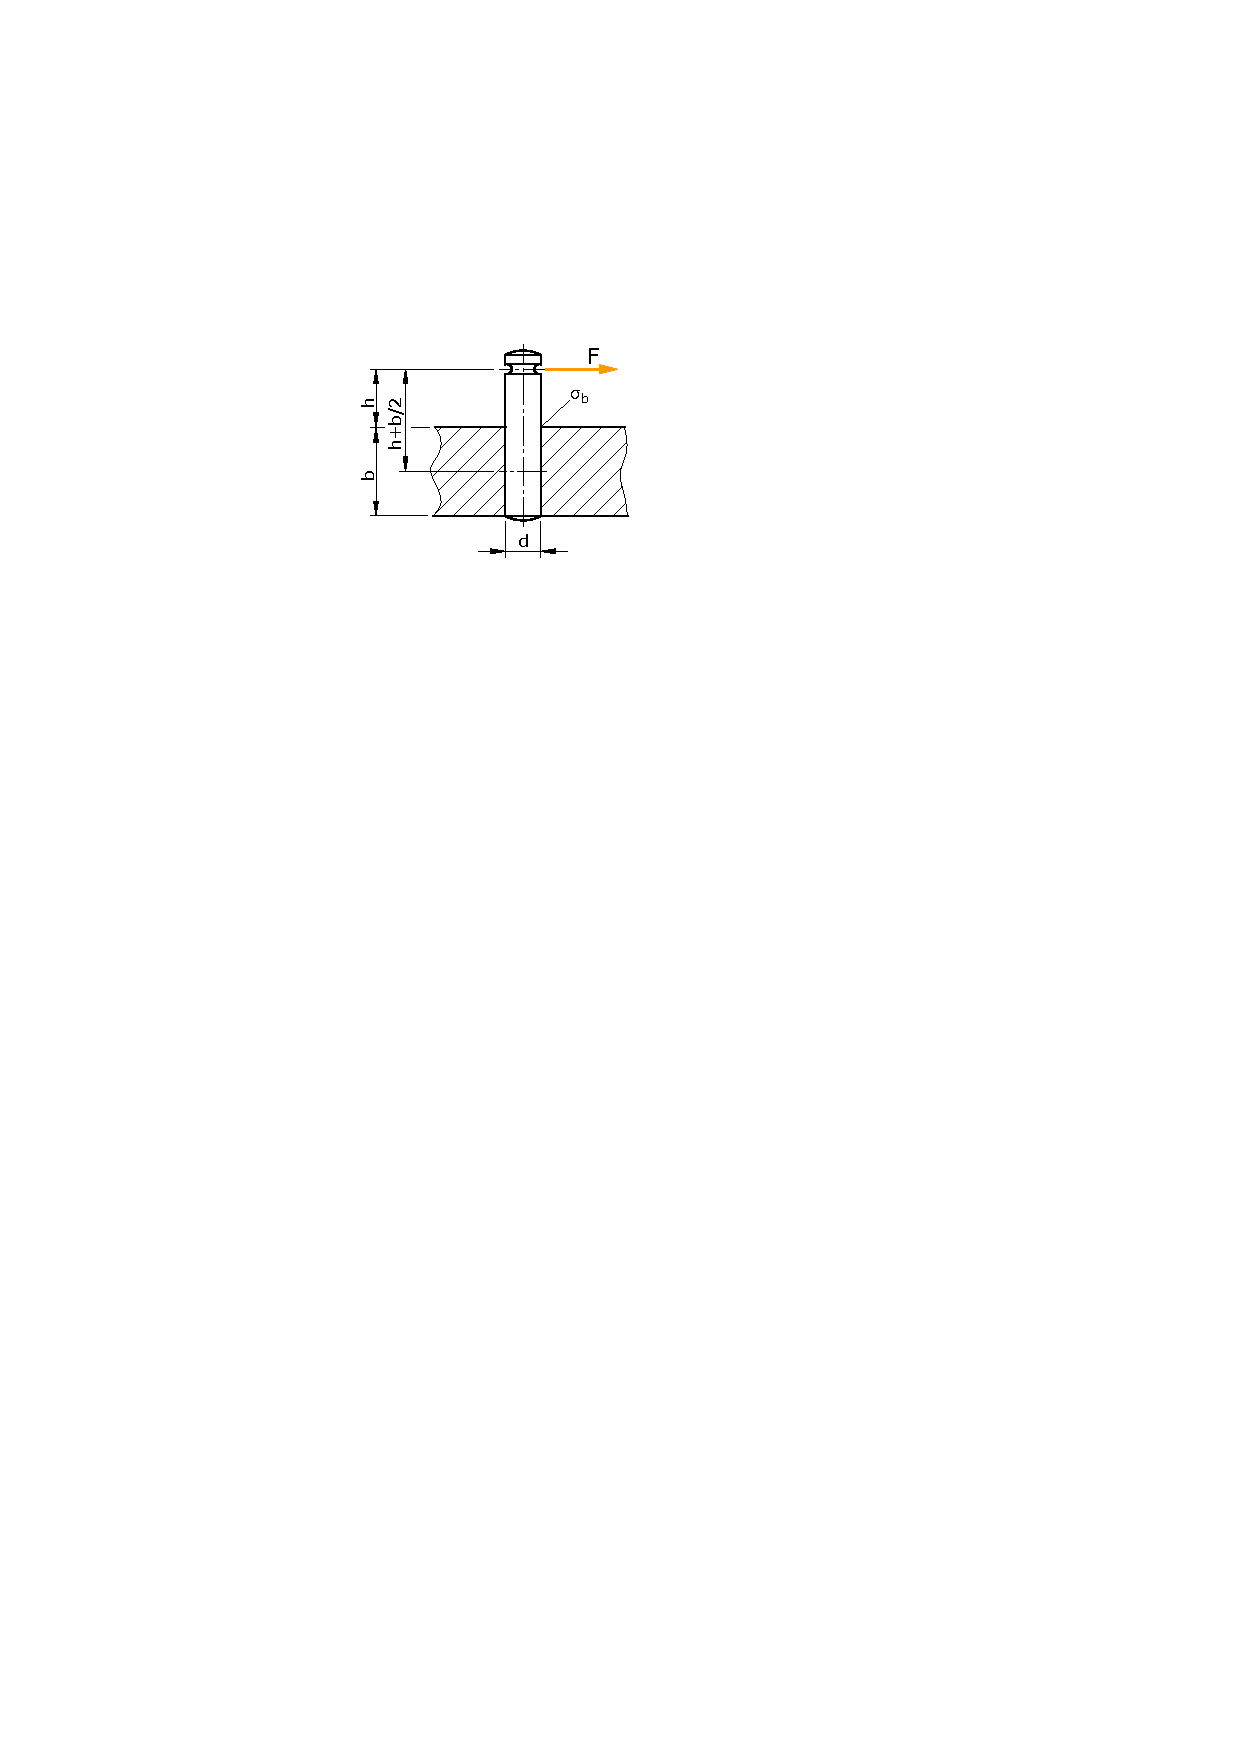
\includegraphics{graphics/steckstift_quer_1}
		\end{center}
		Modell: \\
		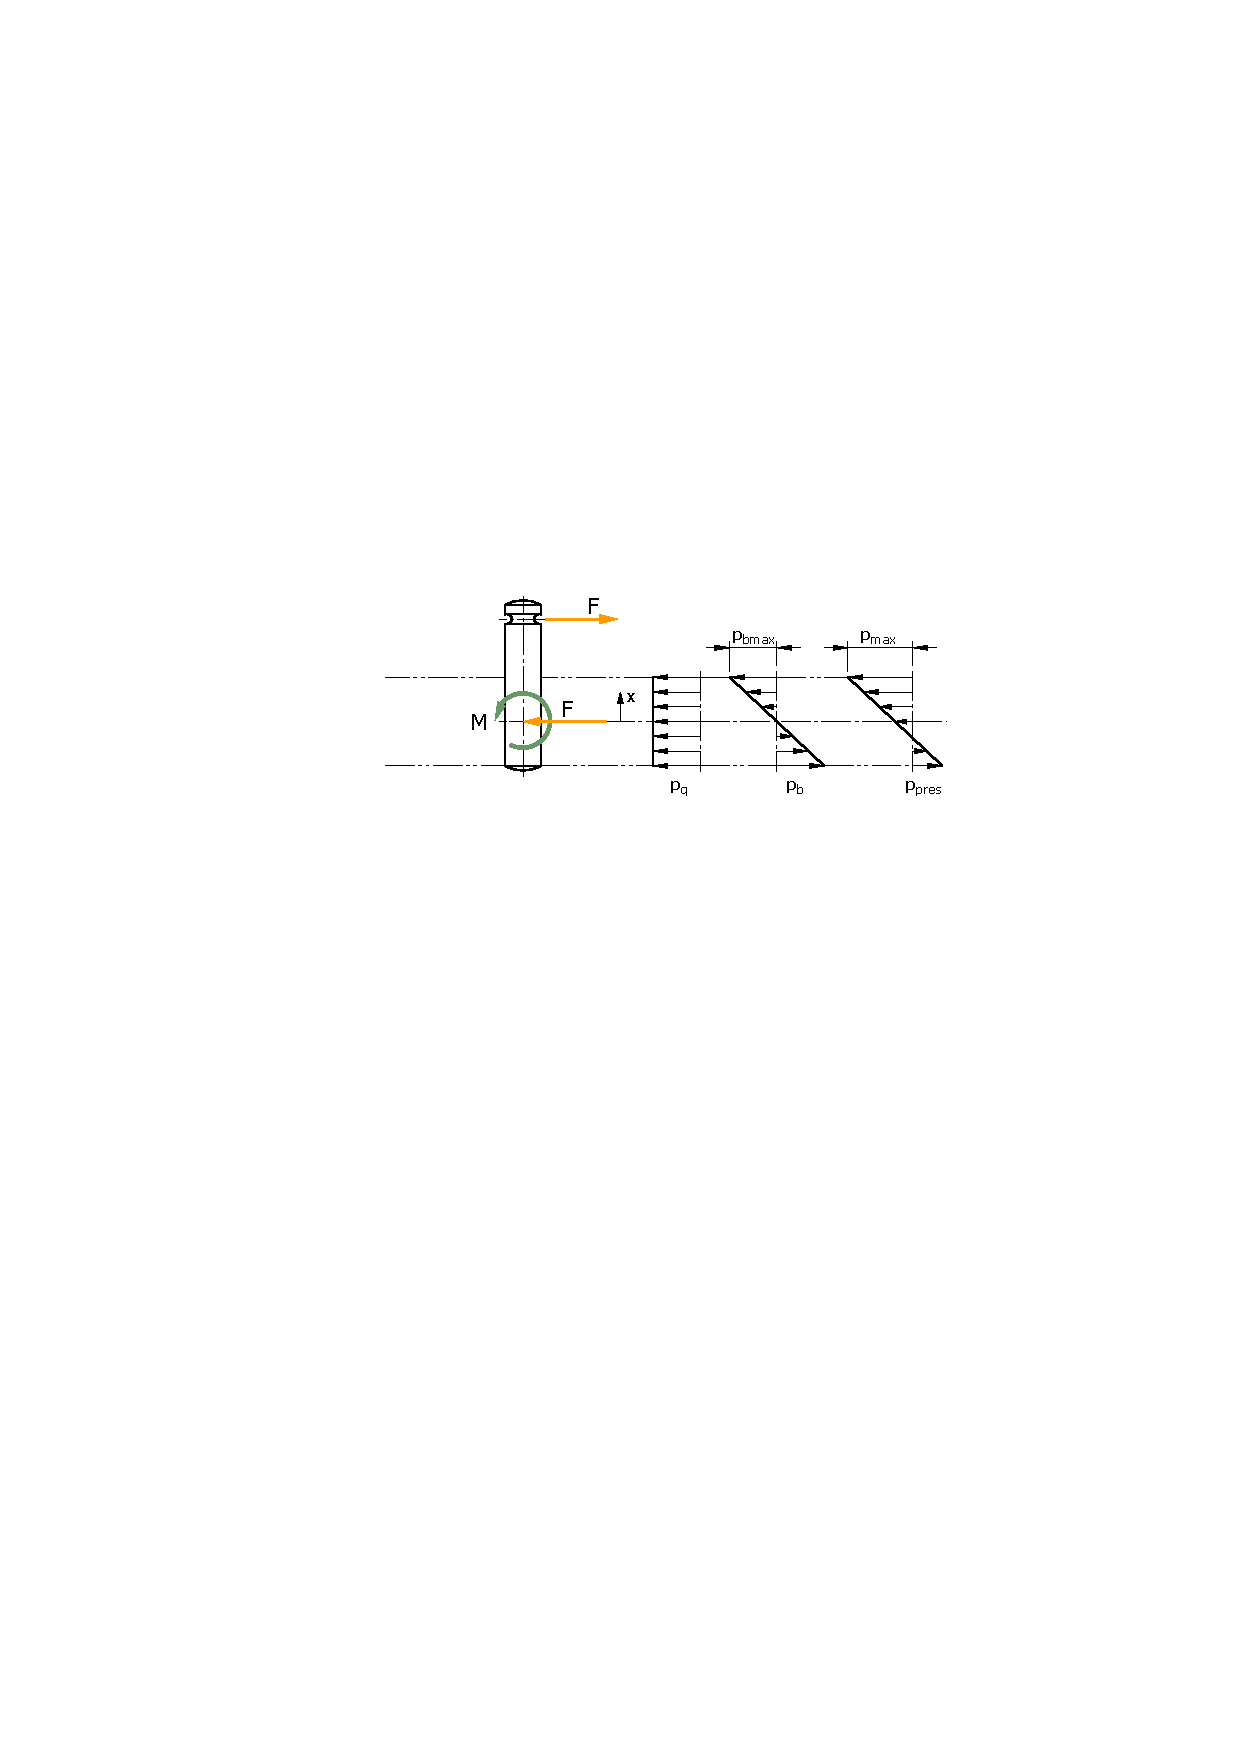
\includegraphics[width=\columnwidth]{graphics/steckstift_quer_2}
		\begin{equation*}
			p_{\text{max}} = p_b + p_q = \frac{4 \cdot F \cdot (1.5 \cdot h + b)}{d \cdot b^2}
		\end{equation*}
		Dimensionierung des Stifts:
		\begin{equation*}
			\sigma_{\text{V}} = \sqrt{\sigma_b^2 + 3 \tau_q^2} < \sigma_{\text{zul}}
		\end{equation*}
		\begin{equation*}
			\text{mit } \sigma_b = \frac{M_b}{W_b}=\frac{32 \cdot F \cdot h}{\pi \cdot d^3}, \quad \tau_q = \frac{F}{A}= \frac{4 \cdot F}{d^2 \cdot \pi}
		\end{equation*}
		Dimensionierung der Bohrung:
		\begin{equation*}
			\sigma_{\text{V}} = - \sigma_z = p_{\text{max}} \leq p_{\text{zul}}
		\end{equation*}
		Für zulässige Festigkeitswerte siehe Anhang \ref{flaechenbelastungen}.
	% subsection: Querkraftbelastete Steckstifte (end)
	\subsection{Querstift mit Drehmomentbelastung} % (fold)
		\begin{center}
			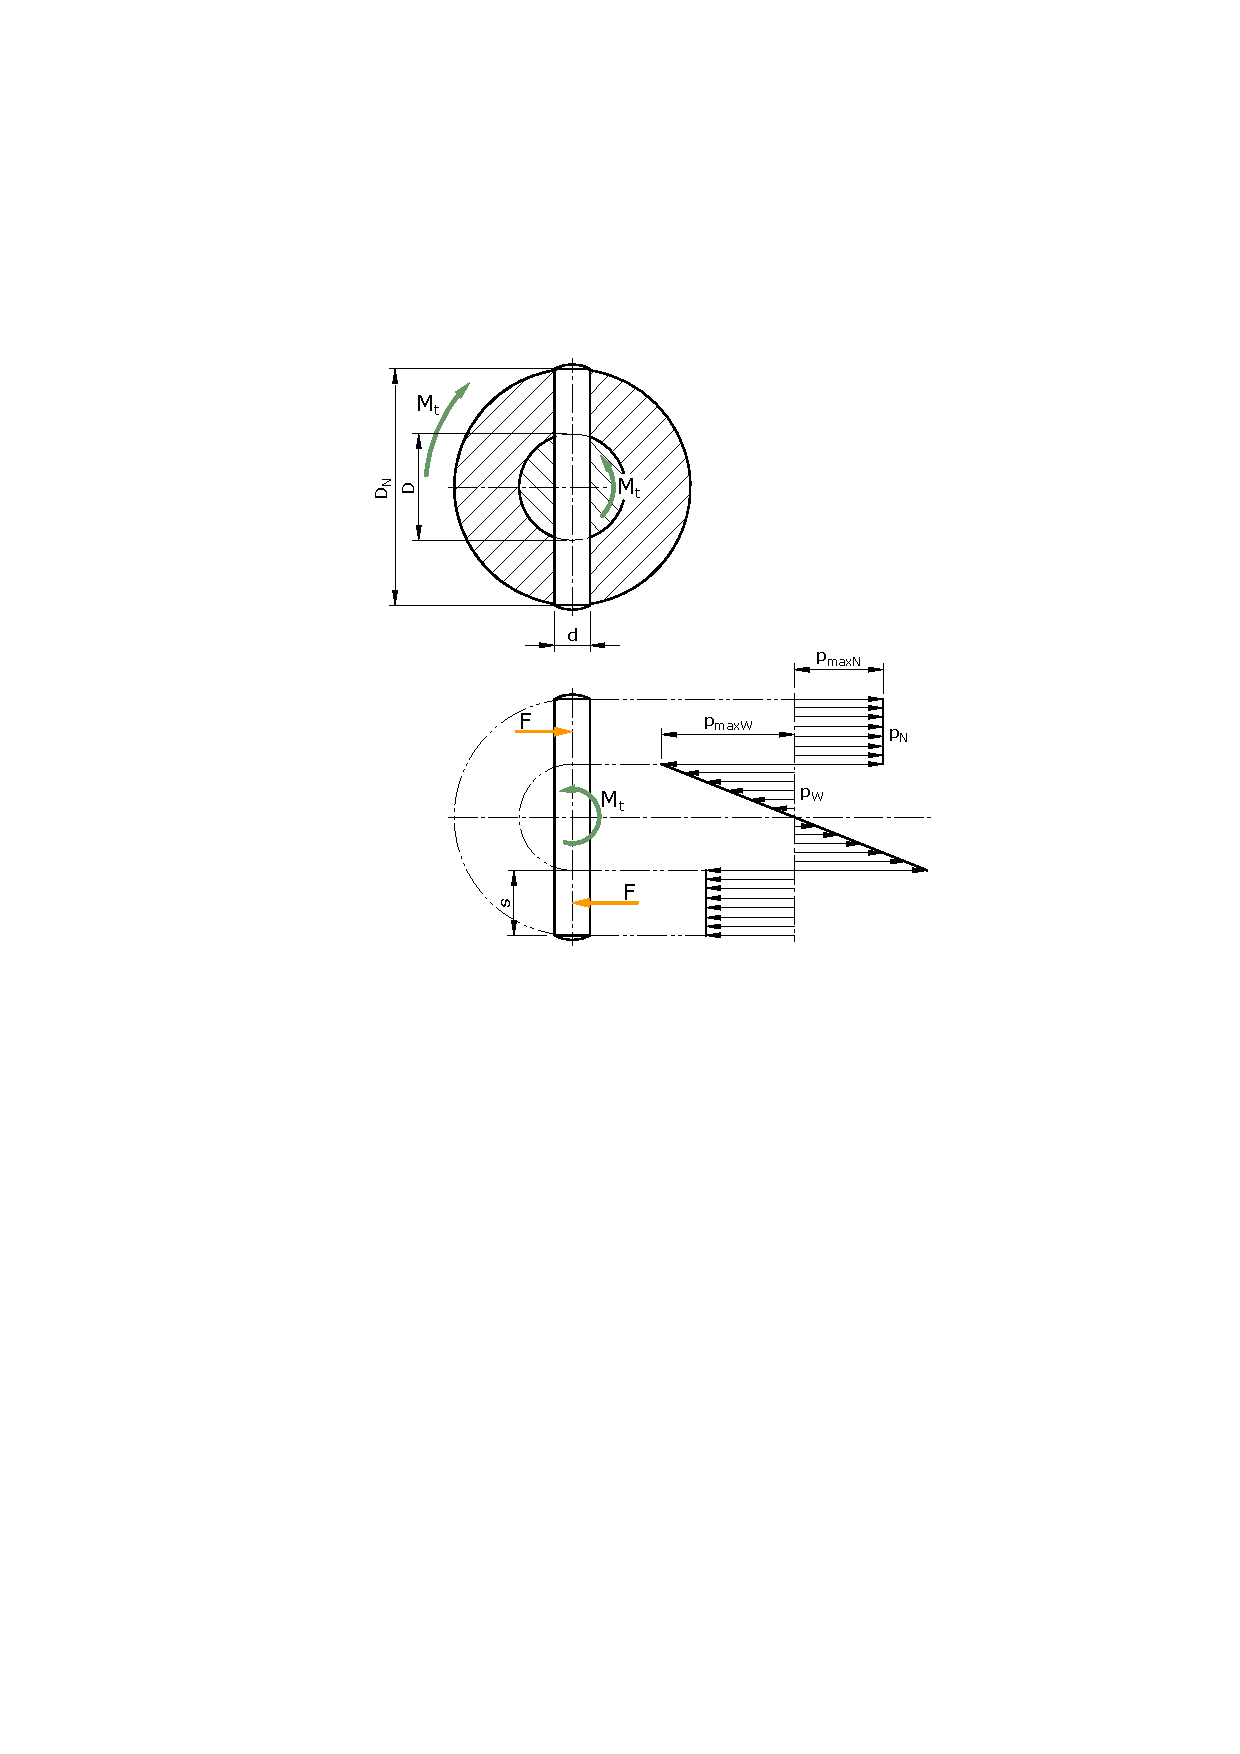
\includegraphics[width=.8\columnwidth]{graphics/querstift_drehmom}
		\end{center}
		\begin{equation*}
			\sigma_{\text{V}} = \sqrt{\sigma_b^2 + 3 \tau_q^2} < \sigma_{\text{zul}}
		\end{equation*}
		\begin{equation*}
			\text{mit } \sigma_b = \frac{M_b}{W_b}= \frac{16 \cdot M_t \cdot s}{D \cdot d^3 \cdot \pi}, \quad \tau_q = \frac{F}{A} = \frac{4 \cdot M_t}{D \cdot \pi \cdot d^2}
		\end{equation*}
		Flächenpressung der Bohrung von Nabe und Welle:
		\begin{equation*}
			p_{\text{maxN}} < p_{\text{zulN}}, \quad p_{\text{maxW}}< p_{\text{zulW}}
		\end{equation*}
		\begin{equation*}
			\text{mit } p_{\text{maxN}} = \frac{4 \cdot M_t}{d \cdot (D_N^2 - D^2)}, \quad p_{\text{maxW}} = \frac{6 \cdot M_t}{d \cdot D^2}
		\end{equation*}
	% subsection: Querstift mit Drehmomentbelastung (end)
	\subsection{Längsstift mit Drehmomentbelastung} % (fold)
		Dimensionierung des Stiftes:
		\begin{equation*}
			\sigma_{\text{V}} = \sqrt{\sigma_z^2 + 3 \tau_q^2} < \sigma_{\text{zul}}
		\end{equation*}
		\begin{equation*}
			\text{mit } \sigma_z = -p = -\frac{4 \cdot M}{d \cdot l \cdot D}, \quad \tau_q = \frac{p}{2} = \frac{2 \cdot M}{D \cdot d \cdot l}
		\end{equation*}
		Dimensionierung der Bohrung:
		\begin{equation*}
			p < p_{\text{zulN}}, \quad p< p_{\text{zulW}}
		\end{equation*}
		Für zulässige Festigkeitswerte siehe Anhang~\ref{flaechenbelastungen}.
		\begin{center}
			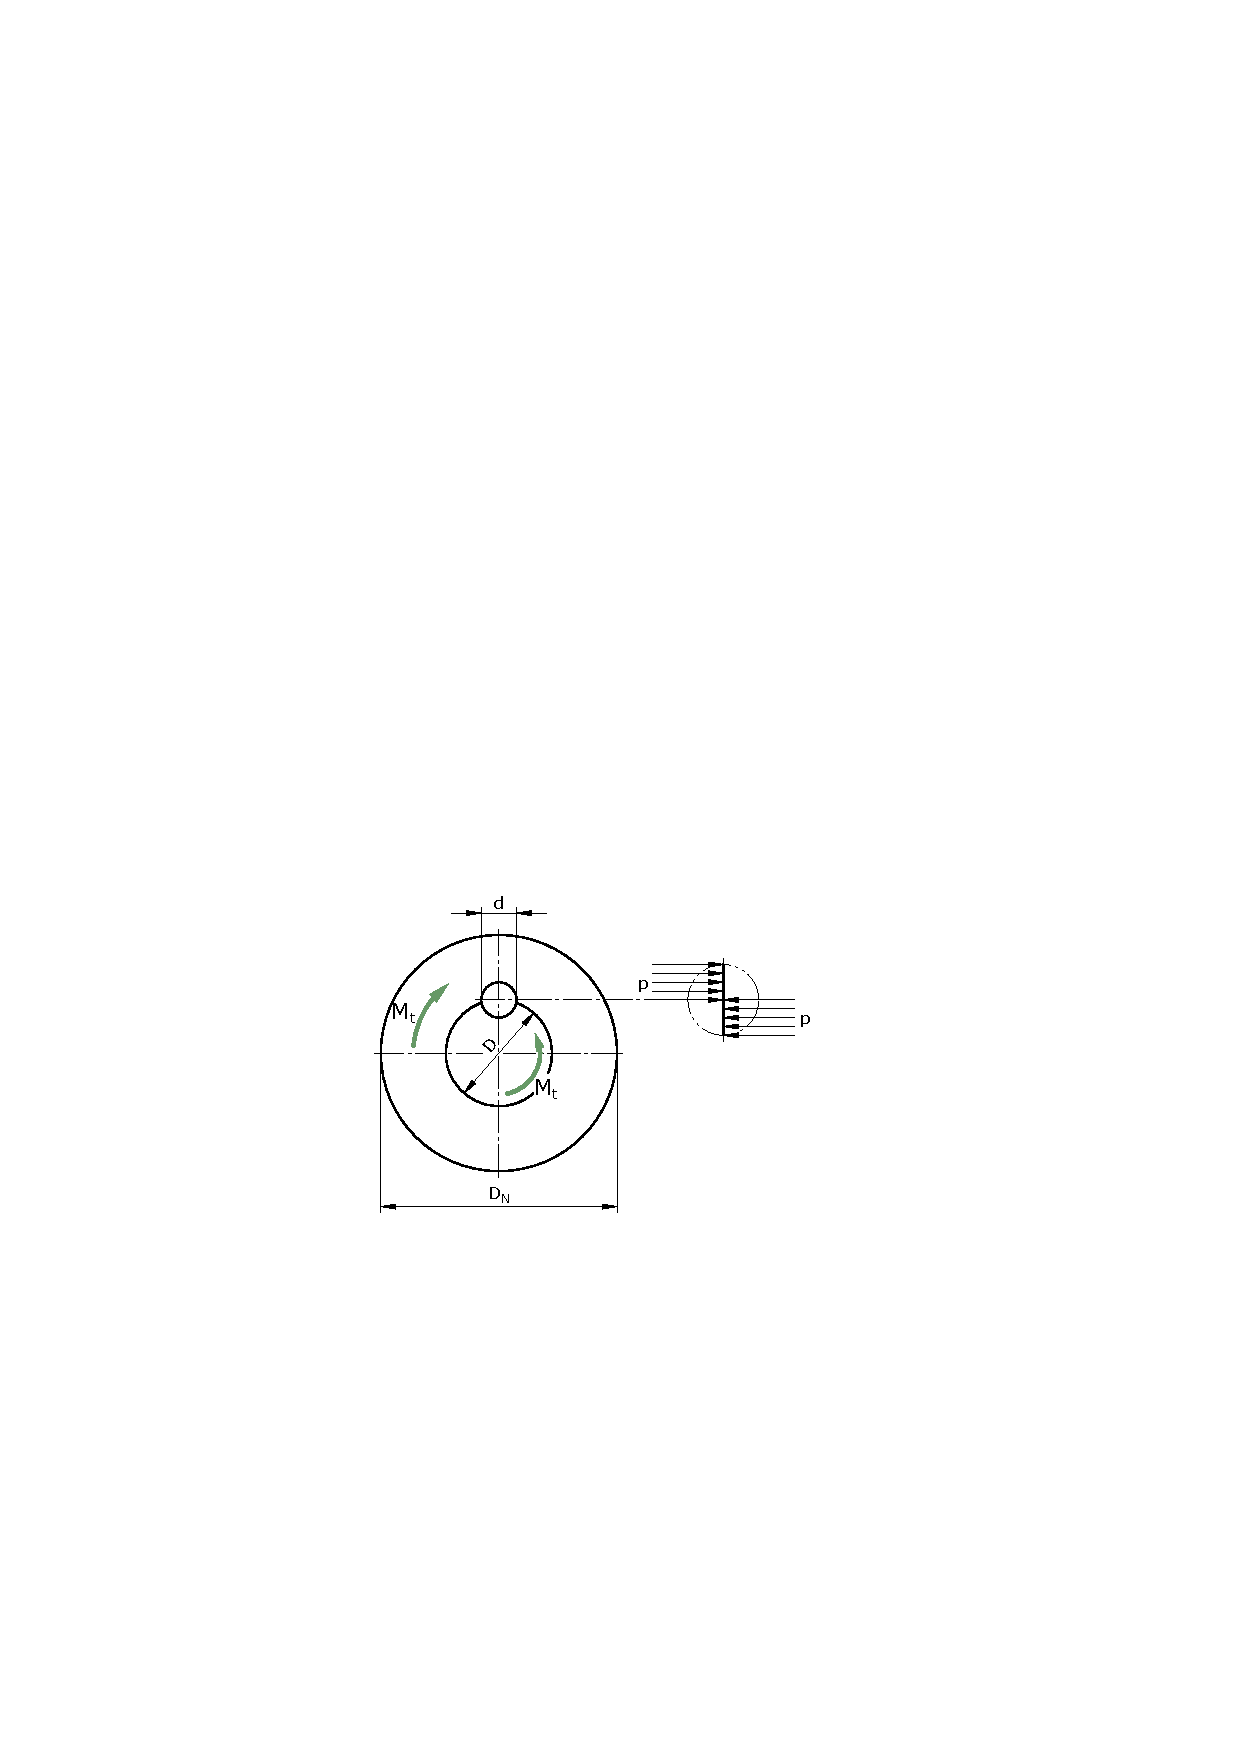
\includegraphics[width=.75\columnwidth]{graphics/laengsstift_drehmom}
		\end{center}
	% subsection: Längsstift mit Drehmomentbelastung (end)
	\subsection{Flanschstift mit Drehmomentbelastung} % (fold)
		\begin{center}
			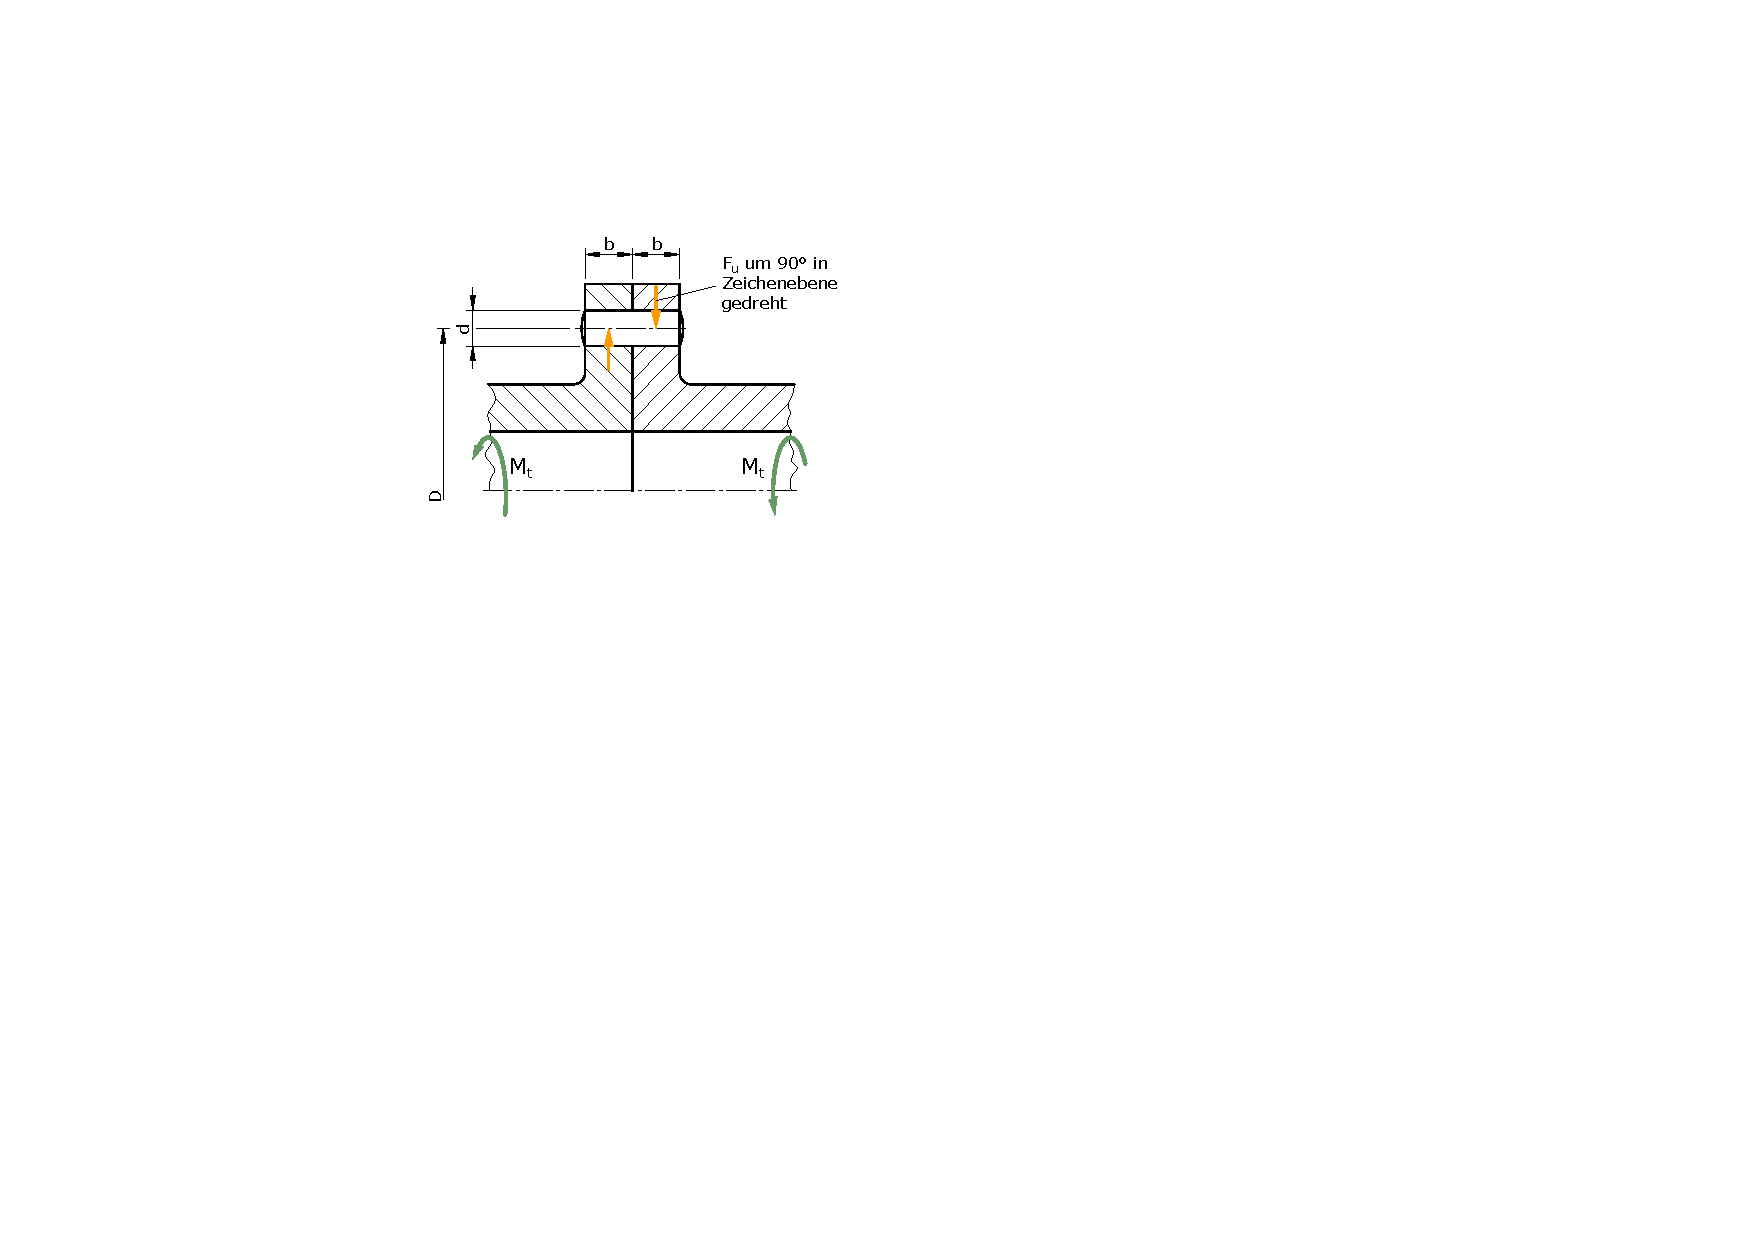
\includegraphics[width=.75\columnwidth]{graphics/flanschstift_drehmom}
		\end{center}
		\begin{equation*}
			\sigma_{\text{V}} = 2 \cdot \tau_q < \sigma_{\text{zul}}, \quad \text{mit } \tau_q = \frac{4 \cdot F_U}{d^2 \cdot \pi}
		\end{equation*}
		\begin{equation*}
			\text{Umfangskraft pro Stift: } F_U = \frac{2 \cdot M_t}{D \cdot z}
		\end{equation*}
		\begin{equation*}
			\text{Flächenpressung: } p_U = \frac{F_U}{b \cdot d}
		\end{equation*}
		Für zulässige Festigkeitswerte siehe Anhang \ref{flaechenbelastungen}.
	% subsection: Flanschstift mit Drehmomentbelastung (end)
	\subsection{Stangen-, Gabel- bzw. Bolzenverbindung} % (fold)
		Entwurfsrichtlinien:
		\begin{center}
			\begin{tabular}{ccc}
				\toprule
				& \textbf{Gleitende Paarung} & \textbf{Feste Paarung} \\
				\midrule
				$\displaystyle\nicefrac{t_S}{d}$ & 1.6 & 1.0 \\
				$\displaystyle\nicefrac{t_G}{d}$ & 0.6 & 0.5 \\
				\bottomrule
			\end{tabular}
		\end{center}

		\begin{center}
			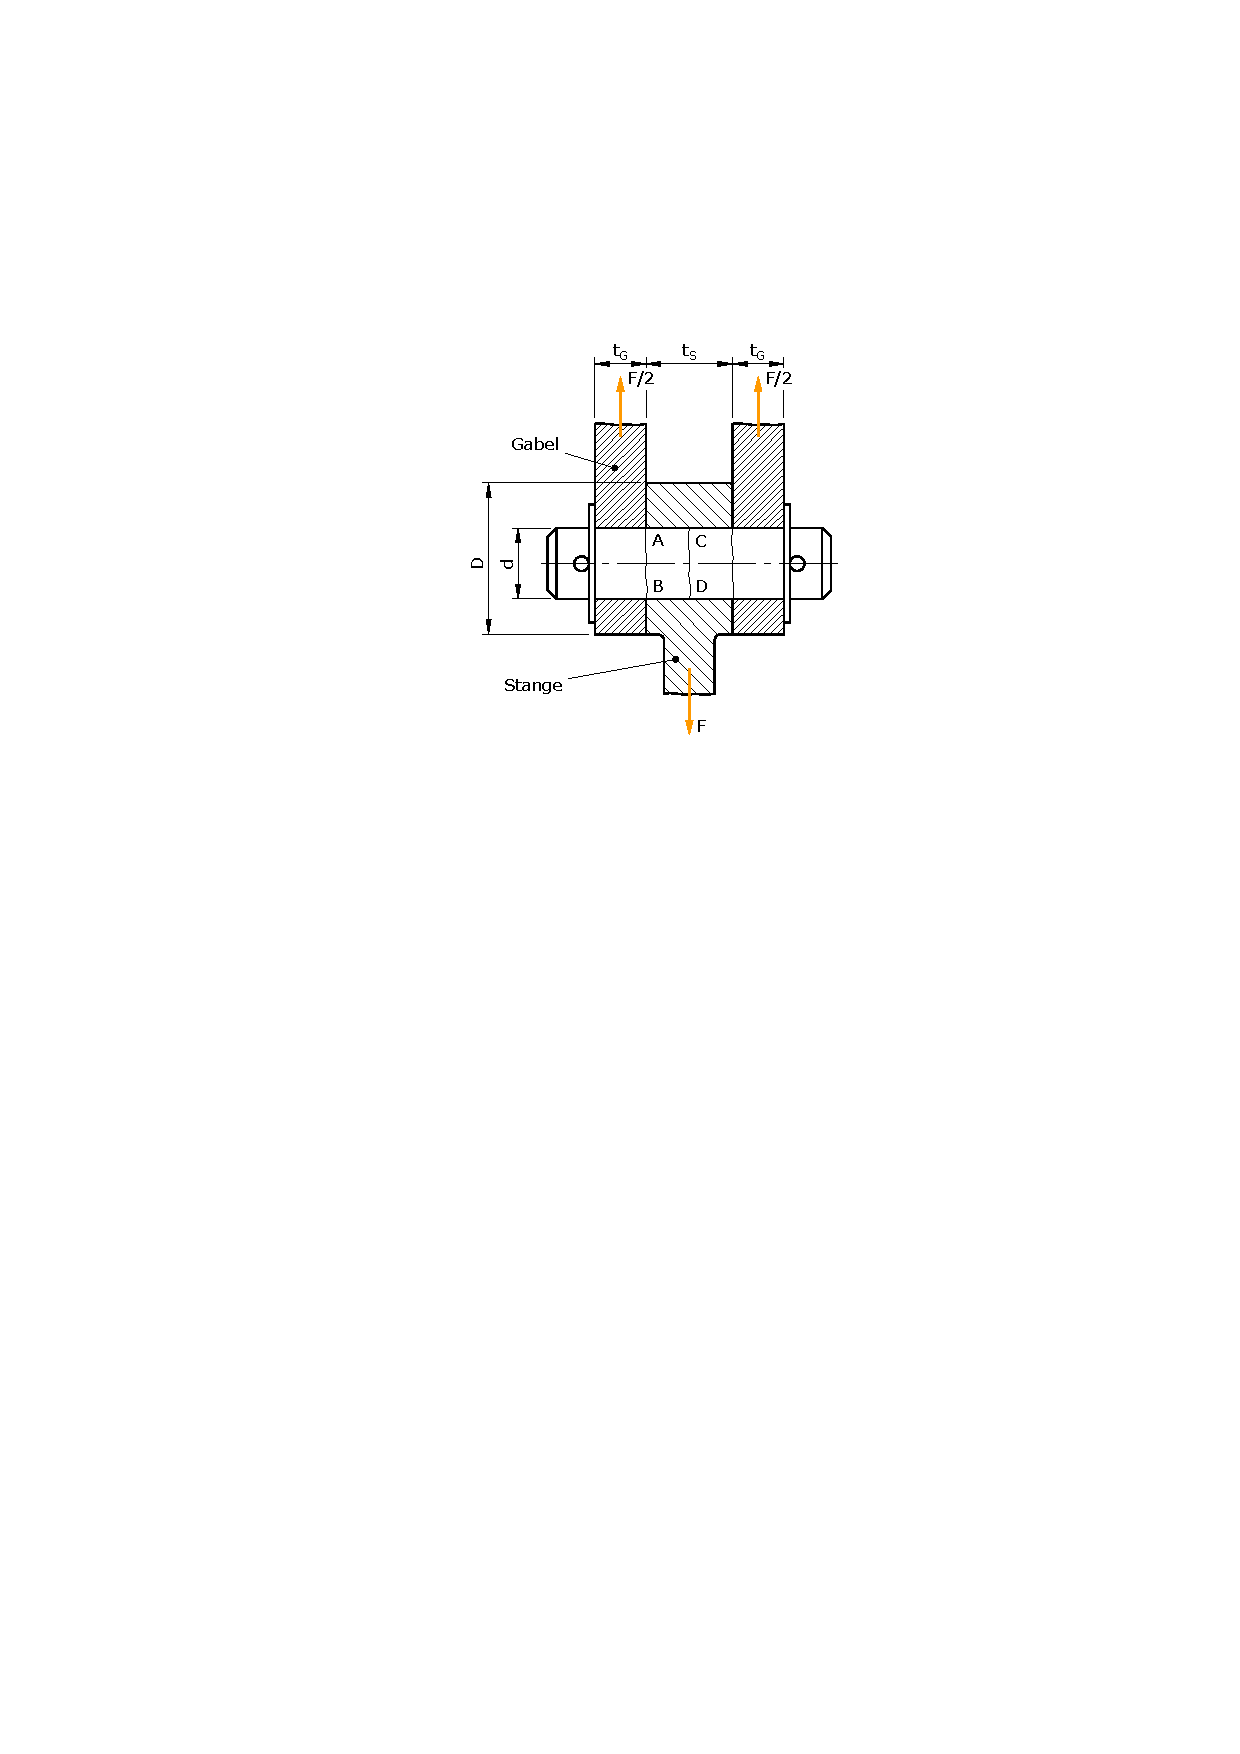
\includegraphics[width=.65\columnwidth]{graphics/stangegabelbolzen}
		\end{center}
		Modellierung: \\
		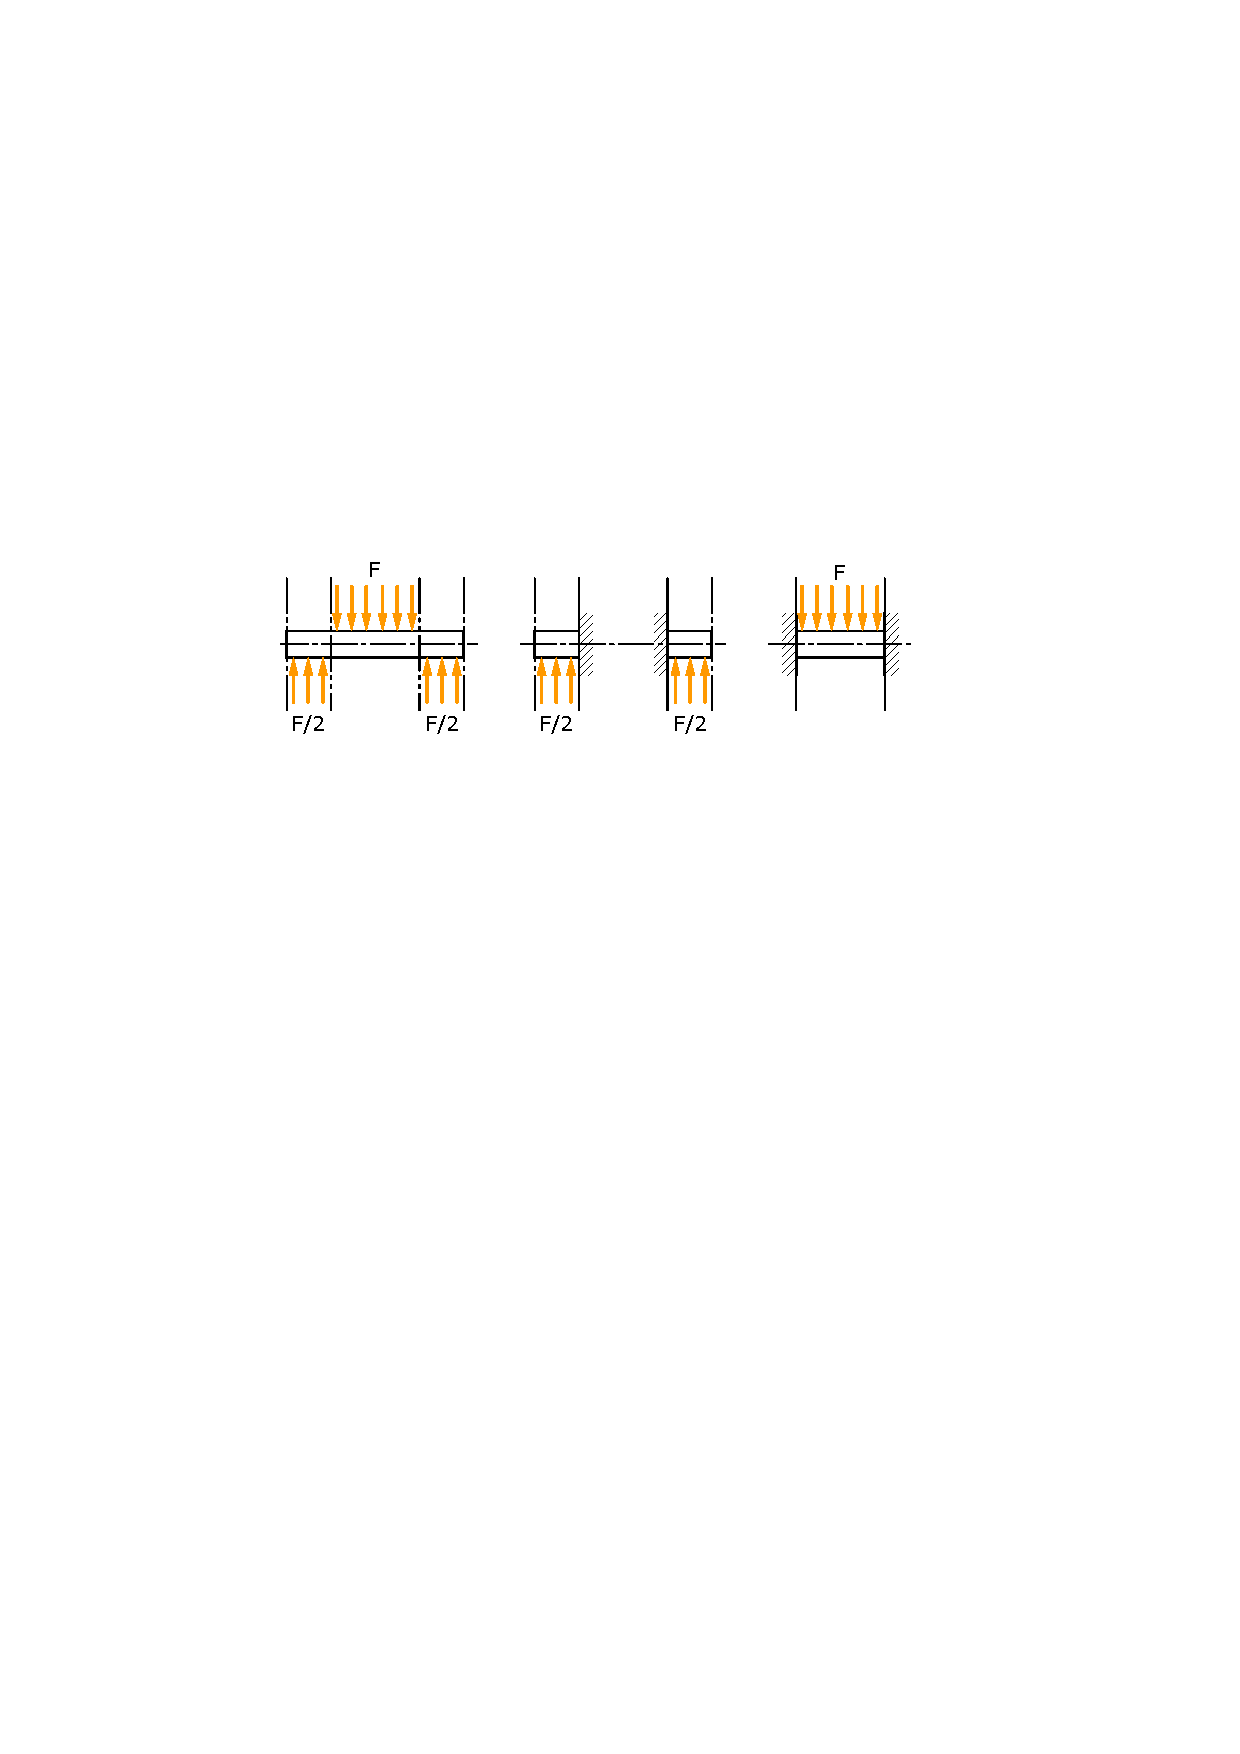
\includegraphics[width=\columnwidth]{graphics/stangegabelbolzen2}
		\begin{tabular}{p{.3\columnwidth}p{.3\columnwidth}p{.3\columnwidth}@{}}
		Bolzen in Stange und Gabel aufliegend & Bolzen in Stange starr eingespannt & Bolzen in Gabel starr eingespannt
		\end{tabular}
		
		Kritischer Querschnitt A -- B:
		\begin{equation*}
			\sigma_{\text{V}} = \sqrt{\sigma_x^2 + 3 \tau_{xy}^2} < \sigma_{\text{zul}}
		\end{equation*}
		\begin{equation*}
			\text{mit } \sigma_x = \frac{M_{\text{b,A--B}}}{W_y}= \frac{8 \cdot F \cdot t_G}{d^3 \cdot \pi}, \quad \tau_{xy}= \frac{\frac{F}{2}}{A}= \frac{2 \cdot F}{d^2 \cdot \pi}
		\end{equation*}
		Kritischer Querschnitt C -- D:
		\begin{equation*}
			\sigma_{\text{V}} = \sigma_x < \sigma_{\text{zul}}, \quad \text{mit } \sigma_x = \frac{M_{\text{b,C--D}}}{W_y}=\frac{8 \cdot F \cdot \left(t_G + \frac{t_S}{2}\right)}{d^3 \cdot \pi}
		\end{equation*}
		Flächenpressung für Gabel / Stange:
		\begin{equation*}
			p_G = \frac{F}{2 \cdot t_G \cdot d} < p_{\text{zul,}G}, \qquad p_S = \frac{F}{t_S \cdot d} < p_{\text{zul,}S}
		\end{equation*}
		Für zulässige Festigkeitswerte siehe Anhang \ref{flaechenbelastungen}.
	% subsection: Stangen-, Gabel- bzw. Bolzenverbindung (end)
% section: Stift- und Bolzenverbindungen (end)